\documentclass[conference]{IEEEtran}
\usepackage{graphicx}
\usepackage{booktabs}
\usepackage{tabularx}
\usepackage[hidelinks]{hyperref}
\urlstyle{same}
\renewcommand{\ttdefault}{cmtt}

\hypersetup{pdftitle={Private Network Service Platform},
  pdfauthor={Aryan Kinha, Divyanshu Singh, Jatin Verma, and Jatin Kumar Singh},
  pdfsubject={Computer Networks course project}}

\begin{document}
\title{Private Network Service Platform\\
Resilient HTTPS on a Four-Mac Local Network}
\author{\IEEEauthorblockN{Aryan Kinha, Divyanshu Singh, Jatin Verma, and Jatin Kumar Singh}
\IEEEauthorblockA{Computer Networks Course Project}}
\maketitle

\begin{abstract}
This project delivers a private HTTPS application on four macOS hosts using
dnsmasq for name resolution, nginx for TLS termination and reverse proxying,
and two independent Flask backends. Verification combined protocol captures,
HTTP header checks, and controlled faults. Both DNS servers returned matching
records with a 30-second time to live (TTL). Both HTTPS edges alternated backend
responses, cache revalidation returned HTTP 304, and eight requests succeeded
through the surviving backend during the outage test. Backup DNS, DNS cutover,
and fault recovery were demonstrated. Backend firewall isolation, client DNS
misconfiguration recovery, and the full directed ping matrix remain open checks.
\end{abstract}

\begin{IEEEkeywords}
DNS, TLS, HTTP caching, load balancing, high availability, packet analysis
\end{IEEEkeywords}

\section{Design and Deployment}

The platform runs entirely on the local network. Table~\ref{tab:roles} assigns
each role, and Fig.~\ref{fig:topology} shows the available paths. The controller
on Mac~1 renders node-specific dnsmasq, nginx, and firewall configurations from a
local inventory, stages them over authenticated SSH, validates them, and
preserves the previous configuration for rollback. The repository provides
the service scripts, configuration templates, and deployment and demo guides
\cite{repo}.

\begin{table}[!b]
\caption{Host Roles and Service Ports}
\label{tab:roles}
\centering
\begin{tabularx}{\columnwidth}{@{}l X@{}}
\toprule
\textbf{Host} & \textbf{Role and listener} \\
\midrule
Mac 1 & Controller, client, primary dnsmasq (UDP/TCP 53) \\
Mac 2 & Backup dnsmasq (53), primary nginx (TCP 80/443) \\
Mac 3 & Standby nginx (TCP 80/443), Backend A (TCP 3001) \\
Mac 4 & Client, Backend B (TCP 3002) \\
\bottomrule
\end{tabularx}
\end{table}

\begin{figure*}[!t]
\centering
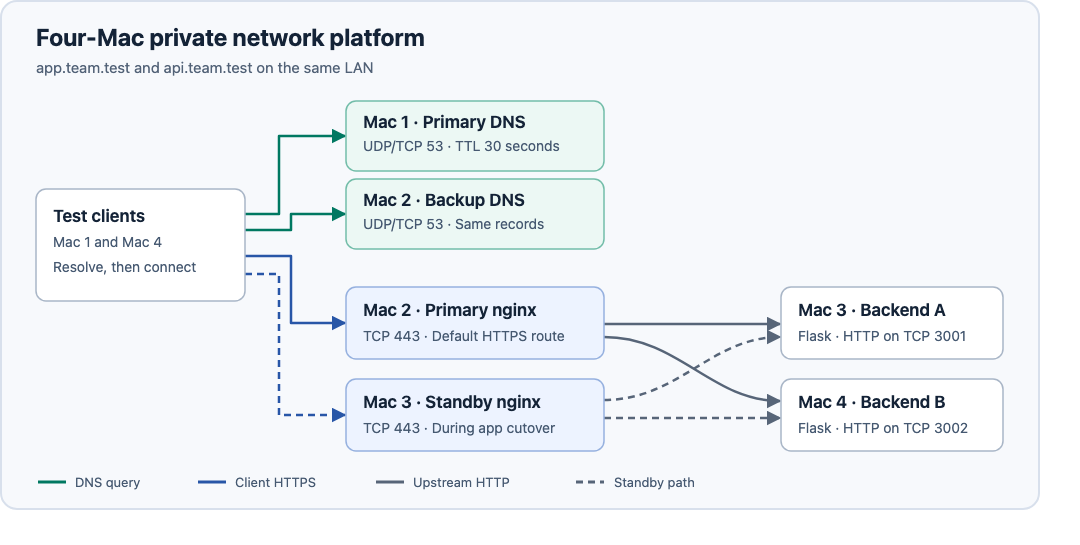
\includegraphics[width=.88\textwidth]{figures/topology.png}
\caption{Four-Mac topology. Dashed paths show standby use during controlled
cutover. Backend A is local to the standby edge. Backend B runs on Mac 4.}
\label{fig:topology}
\end{figure*}

Both resolvers advertise the primary edge for the private service names in Fig.~\ref{fig:topology}, with TTL 30~s \cite{dns}.
After DNS, the client opens a
separate TCP connection and validates the TLS certificate for the requested
name \cite{tcp,tls}. Both edges serve the same team certificate with both DNS
names in its subject alternative names. nginx redirects HTTP to HTTPS at
the edge and forwards plain HTTP to the selected backend. The Flask
\texttt{/api/status} response identifies A or B in \texttt{X-Backend}. nginx adds
\texttt{X-Edge}. The \texttt{/api/cache} endpoint uses a shared representation
and ETag, with \texttt{Cache-Control: public, max-age=60}. A matching
\texttt{If-None-Match} yielded 304 \cite{cache}.

\section{Verification and Fault Recovery}

The 24 November 2026 LAN capture ties the DNS answer to the client-to-edge TCP
and TLS exchanges (Table~\ref{tab:frames}). The TLS~1.2 certificate handshake
message is visible in this capture. The application records are encrypted, so
curl output supplies the HTTP status and headers independently. Directed ping
succeeded in nine of twelve directions. All three failures targeted Mac~1,
which had stealth mode enabled. The confirmed team-resolver client outside
Mac~1 was Mac~4. Traces, screenshots, and terminal output are indexed in the
\href{https://github.com/aryankinha/cn-project/blob/main/docs/submission.md}{submission evidence}.

\begin{table}[!b]
\caption{Observed Packet Sequence on the Client LAN}
\label{tab:frames}
\centering
\begin{tabularx}{\columnwidth}{@{}l X@{}}
\toprule
\textbf{Frame(s)} & \textbf{Observed event} \\
\midrule
1, 2 & DNS A query and answer, TTL 30~s \\
3--5 & TCP SYN, SYN-ACK, ACK, destination port 443 \\
6, 9 & TLS 1.2 ClientHello, then ServerHello and Certificate \\
11, 13 & TLS ChangeCipherSpec and encrypted handshake records \\
15, 17 & Encrypted TLS application data in both directions \\
\bottomrule
\end{tabularx}
\end{table}

\subsection{Resolver Availability and TTL}
With the primary resolver stopped, a fresh Mac~4 lookup received a captured
reply from backup DNS and ordinary HTTPS returned 200. The primary resolver
then recovered. In the TTL test, the client initially retained its old answer
after both resolvers changed. The new answer appeared after expiry. A separate
authorized cache flush immediately exposed the restored primary address.
Direct resolver queries and client-system lookups identified the authoritative
record and the cached answer respectively.

\subsection{Backend Isolation and Failover}
A dedicated macOS \texttt{pf} anchor scopes the two backend policy files. The
strict profile allows the primary edge and local traffic to Backend A. The
standby profile additionally permits Mac~3 to reach Backend B. Syntax
validation passed. Both ports remained directly reachable from Mac~1 during
the recorded probes, so live denial and rollback still require owner-assisted
verification. With Backend~A stopped, all eight requests returned HTTP 200
from B. A rejoined after restart and A/B rotation resumed. Passive retries
kept a backend outage within the current edge. Moving clients away from a
failed edge address requires a separate mechanism.

\subsection{Edge Cutover and Fault Diagnosis}
Both resolvers changed only the application record during cutover. A cached
client initially reached the primary edge and a fresh client reached the
standby, as shown by \texttt{X-Edge}. The application record was restored and
clients converged back to the primary. The wrong-record, one-backend-down,
both-backends-down, and wrong-port scenarios were observed. With both backends
down, DNS and TLS still worked and nginx returned 502. A deliberate wrong
client DNS setting and its recovery remain to be demonstrated.

The troubleshooting drill located a stopped edge at the TCP layer. A subsequent
502 showed that TLS was working while nginx workers could not reach the
upstreams. Direct probes from the edge host isolated the failure to the worker
path. Starting nginx from the logged-in owner's session restored upstream
access. The verification order was DNS, TCP, TLS, HTTP, and backend reachability.

\newpage
\section{Conclusion}

The recorded tests establish trusted named access, end-to-end protocol
visibility, caching, resolver failover, backend recovery, and controlled edge
migration on four hosts. The standby reduces dependence on the primary edge
during a planned cutover. Automatic edge failover would require an independent
health decision and a way to move traffic beyond the existing DNS cache window.
The remaining live checks are firewall denial and rollback, wrong-client-DNS
recovery, and the full reachability matrix.

\begin{thebibliography}{00}
\bibitem{repo}
A. Kinha, D. Singh, J. Verma, and J. K. Singh,
\emph{Private Network Service Platform}, GitHub repository, Nov. 2026.
[Online]. Available: \url{https://github.com/aryankinha/cn-project}
\bibitem{dns}
P. Mockapetris, \emph{Domain Names---Implementation and Specification},
RFC 1035, Nov. 1987. doi: 10.17487/RFC1035.
\bibitem{tcp}
W. Eddy, Ed., \emph{Transmission Control Protocol (TCP)},
RFC 9293, Aug. 2022. doi: 10.17487/RFC9293.
\bibitem{tls}
E. Rescorla, \emph{The Transport Layer Security (TLS) Protocol Version 1.3},
RFC 8446, Aug. 2018. doi: 10.17487/RFC8446.
\bibitem{cache}
R. Fielding, M. Nottingham, and J. Reschke,
\emph{HTTP Caching}, RFC 9111, Jun. 2022. doi: 10.17487/RFC9111.
\end{thebibliography}
\end{document}
